\documentclass{beamer}
\mode<presentation>
\usetheme{Warsaw}
\setbeamertemplate{headline}{}
\usepackage{subcaption}
\usepackage{empheq}
\usepackage{xspace} % Para problemas de espaciado al definir comandos
\usepackage{xurl}
\usepackage{hyperref}
\usepackage{gensymb}
\usepackage{amsmath}

\title{Trabajo de Fin de Grado}
\subtitle{Métodos para la resolución de
	ecuaciones integrales y su
	integración en un sistema
	para la simulación de la
	distribución de temperatura
	en edificios mediante el uso
	de servicios web}
\author{David Cantón Ruiz}
\institute{Universidad de Granada}
\begin{document}
\begin{frame}[plain]
    \maketitle
\end{frame}
\begin{frame}{Indice}
	\tableofcontents
\end{frame}
\section{Introducción}
\begin{frame}{Introducción}
	\begin{equation*}
		u(x) = f(x) + \int_0^x K(x,t)u(t)dt, \qquad x \in [0,B]
	\end{equation*}
	\begin{figure}
		\centering
		\begin{subfigure}[t]{0.3\textwidth}
			
\includegraphics[width=\textwidth]{react}
		\end{subfigure}
		\begin{subfigure}[b]{0.3\textwidth}
			
\includegraphics[width=\textwidth]{python}
		\end{subfigure}
		\begin{subfigure}[b]{0.4\textwidth}
			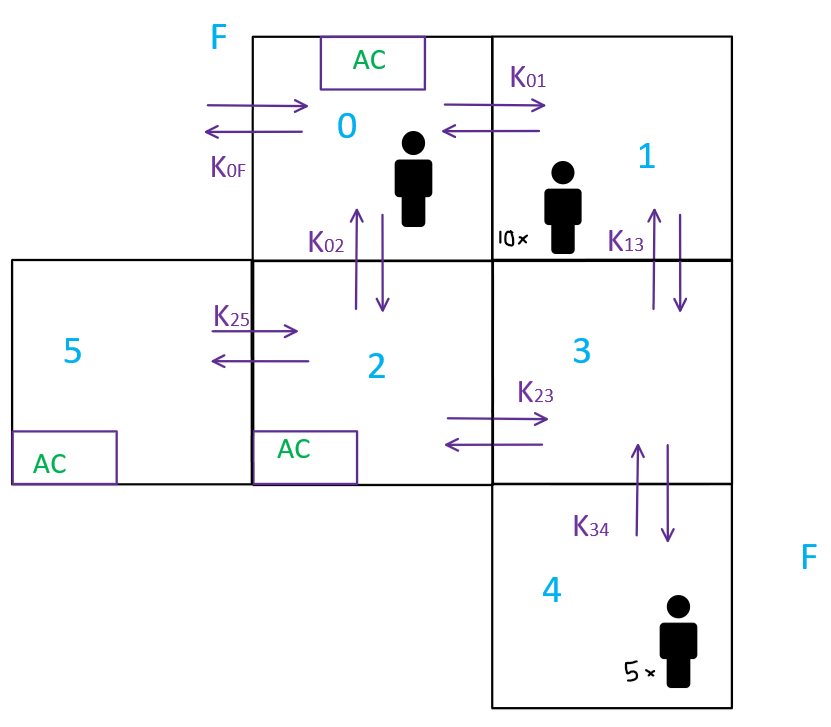
\includegraphics[width=\textwidth]{edificio_6habs}
		\end{subfigure}
	\end{figure}
\end{frame}
\section{Clasificación de ecuaciones integrales}
\begin{frame}{Clasificación de ecuaciones integrales}
	Ecuación integral de Volterra de segunda clase:
\begin{equation*}
	u(x) = f(x) + \int_0^x K(x,t)u(t)dt, \qquad x \in [0,B].
\end{equation*}
\begin{equation*}
	u(x) = 5x + 2\int_0^x (x-t)u(t)dt, \qquad x \in [0,4].
\end{equation*}
Ecuación integral de Fredholm de segunda clase:
\begin{equation*}
	u(x) = f(x) + \int_a^b K(x,t)u(t)dt, \qquad x \in [a,b].
\end{equation*}
\begin{equation*}
	u(x) = \sin x + \dfrac{1}{4}\int_{0}^2 (x-t)u(t)dt, \qquad x \in [0,2].
\end{equation*}
\end{frame}
\section{Existencia y unicidad de solución}
\begin{frame}{Existencia y unicidad de solución}
\begin{itemize}
	\item Teorema de la serie geométrica
	\item Generalización del teorema\\
\end{itemize}
\vspace*{0.5cm}
\begin{equation*}
	(I-L)u = f
\end{equation*}
\vspace*{0.5cm}
\centering
$\Downarrow$
\vspace*{0.2cm}
\begin{itemize}
	\item Toda ecuación integral lineal de Volterra de segunda clase tiene solución única, trabajando en un contexto continuo.
\end{itemize}
\end{frame}
\begin{frame}
	\centering
	\textbf{Caso vectorial}
	\begin{equation*}
		\textbf{u}(x) = \textbf{f}(x) + \int_0^x \textbf{K}(x,t)\textbf{u}(t)dt, \qquad x \in [0,B],
	\end{equation*}
	\begin{equation*}
		\textbf{u}(x) = \begin{pmatrix}	u_1(x) \\ u_2(x) \\ \vdots \\ u_n(x)	\end{pmatrix}, \qquad \textbf{f}(x) = \begin{pmatrix}	f_1(x) \\ f_2(x) \\ \vdots \\ f_n(x)	\end{pmatrix}, \qquad \textbf{K}(x,t) = \begin{pmatrix}	K_1(x,t) \\ K_2(x,t) \\ \vdots \\ K_n(x,t)	\end{pmatrix}.
	\end{equation*}
\end{frame}
\section{Métodos de resolución de ecuaciones integrales de Volterra}
\begin{frame}{Métodos de resolución de ecuaciones integrales de Volterra}
	\framesubtitle{Método de la solución en series (caso escalar)}
	\begin{equation*}
		u(x) = 1 - x \sin x + \int_{0}^{x} tu(t)dt.
	\end{equation*}
	La solución en forma de serie viene dada por
	\begin{equation*}
		u(x) = 1 - \dfrac{1}{2!}x^2 + \dfrac{1}{4!}x^4-\dfrac{1}{6!}x^6+\cdots
	\end{equation*}
	que nos da la solución exacta: $u(x) = \cos x.$
	\begin{figure}[h!]
		\centering
		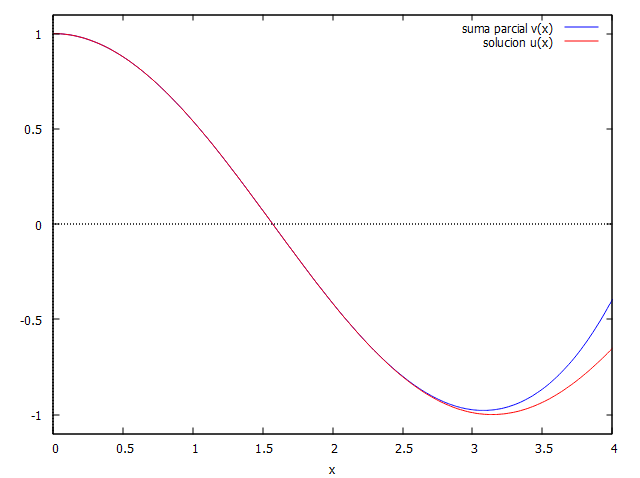
\includegraphics[width=0.5\textwidth]{suma_parcial_sol}
	\end{figure}
\end{frame}
\begin{frame}{Método de aproximaciones sucesivas (caso vectorial)}
	\[ \begin{dcases}
		y(x) = 1 + \displaystyle \int_0^x (\dfrac{1}{8}y(t)-\dfrac{1}{6}v(t))dt \\
		v(x) = 3+ \displaystyle \int_0^x (\dfrac{1}{7}y(t)-\dfrac{1}{8}v(t))dt \;
	\end{dcases} \]%
	\begin{equation*}
		\textbf{u}(x) = \begin{pmatrix}	y(x) \\[6pt] v(x)	\end{pmatrix}, \qquad \textbf{f}(x) = \begin{pmatrix}	1 \\[6pt] 3	\end{pmatrix}, \qquad \textbf{K}(x,t) = \begin{pmatrix}	\dfrac{1}{8} & -\dfrac{1}{6} \\[9pt] \dfrac{1}{7} & -\dfrac{1}{8}	\end{pmatrix},
	\end{equation*}
\begin{equation*}
	\textbf{u}_0 = \begin{pmatrix}	0 \\ 1	\end{pmatrix}.
\end{equation*}
	La fórmula iterativa viene dada por:
	\begin{equation*}
		\textbf{u}_{n+1}(x) = \textbf{f}(x) + \int_0^x \textbf{K}(x,t)\textbf{u}_n(t)dt, \qquad n \geqslant 0.
	\end{equation*}
\end{frame}
\begin{frame}
	\begin{figure}[h!]
		\centering
		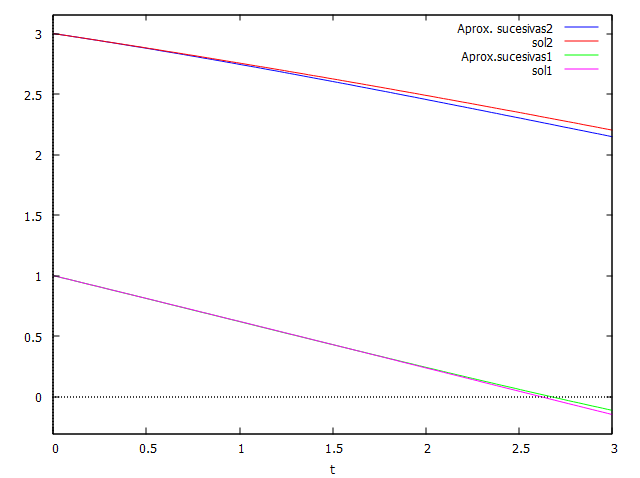
\includegraphics[width=0.8\textwidth]{comp_sol_ej43}
		\caption{Solución exacta y con aproximaciones sucesivas}
	\end{figure}
\end{frame}
\section{Relación entre ecuaciones diferenciales y ecuaciones de Volterra}
\begin{frame}{Relación entre ecuaciones diferenciales y ecuaciones de Volterra}
	Las ecuaciones diferenciales lineales son un caso particular de las ecuaciones de Volterra.
\begin{equation*}
	x \in \mathcal{C}^1(0,B):\left\lbrace\begin{array}{c} x'(t) = a(t)x(t)+b(t) \\ x(0) = x_0 \end{array}\right.,\qquad t \in (0,B).
\end{equation*}
La solución del PVI coincide con la solución de la ecuación integral lineal de Volterra de segunda clase:
\begin{equation*}
	x(t) = f(t) + \int_0^t K(t,s)x(s)ds,
\end{equation*}
donde
\begin{equation*}
	f(t) = x_0 + \int_0^t b(s)ds, \qquad K(t,s) = a(s).
\end{equation*}
\end{frame}
\section{Aplicación: Calentamiento y enfriamiento de edificios}
\begin{frame}{Aplicación: Calentamiento y enfriamiento de edificios}
\begin{figure}[h!]
	\centering
	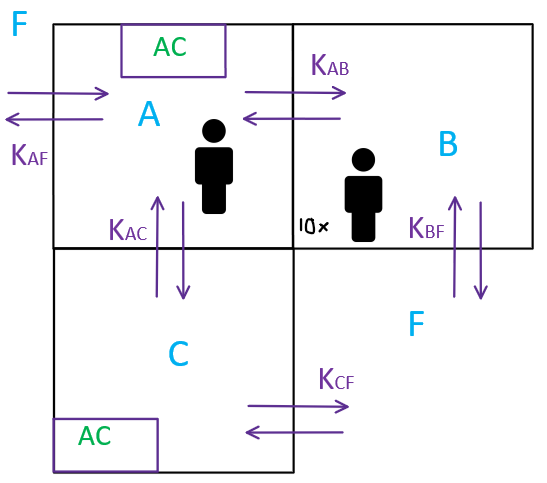
\includegraphics[width=0.4\textwidth]{edificio_3habs}
\end{figure}
\begin{equation}\begin{dcases}
		a'(t)= \dfrac{b(t)-a(t)}{K_{AB}} + \dfrac{c(t)-a(t)}{K_{AC}} + \dfrac{M(t) - a(t)}{K_{AF}} + U(t) + H(t) \\  b'(t)= \dfrac{a(t)-b(t)}{K_{AB}} + \dfrac{M(t) - b(t)}{K_{BF}} + 10H(t) \\ c'(t)= \dfrac{a(t)-c(t)}{K_{AC}} + \dfrac{M(t) - c(t)}{K_{CF}} + U(t) \end{dcases}
\end{equation}
\end{frame}
\begin{frame}
	\begin{equation*}
		a(t_0) = 20 \celsius, \qquad b(t_0) = 10 \celsius, \qquad c(t_0) = 15 \celsius.
	\end{equation*}
	\begin{figure}[h!]
		\centering
		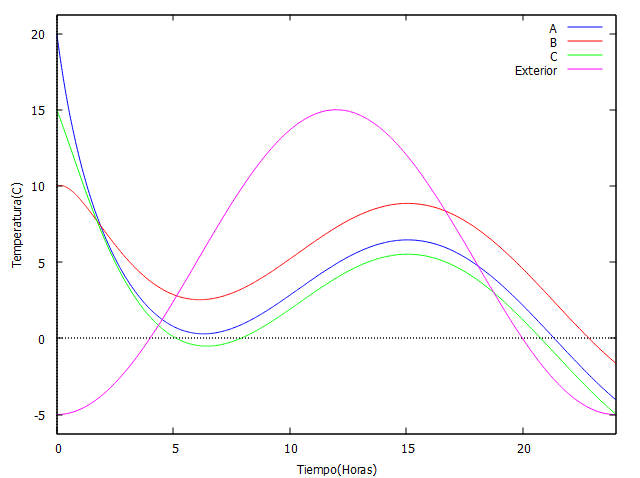
\includegraphics[width=0.8\textwidth]{graf_sol3}
	\end{figure}
\end{frame}
\section{Diseño e implementación}
\begin{frame}{Diseño e implementación}
	\centering
	https://github.com/vaynilla/TFG
\begin{figure}[h!]
	\centering
	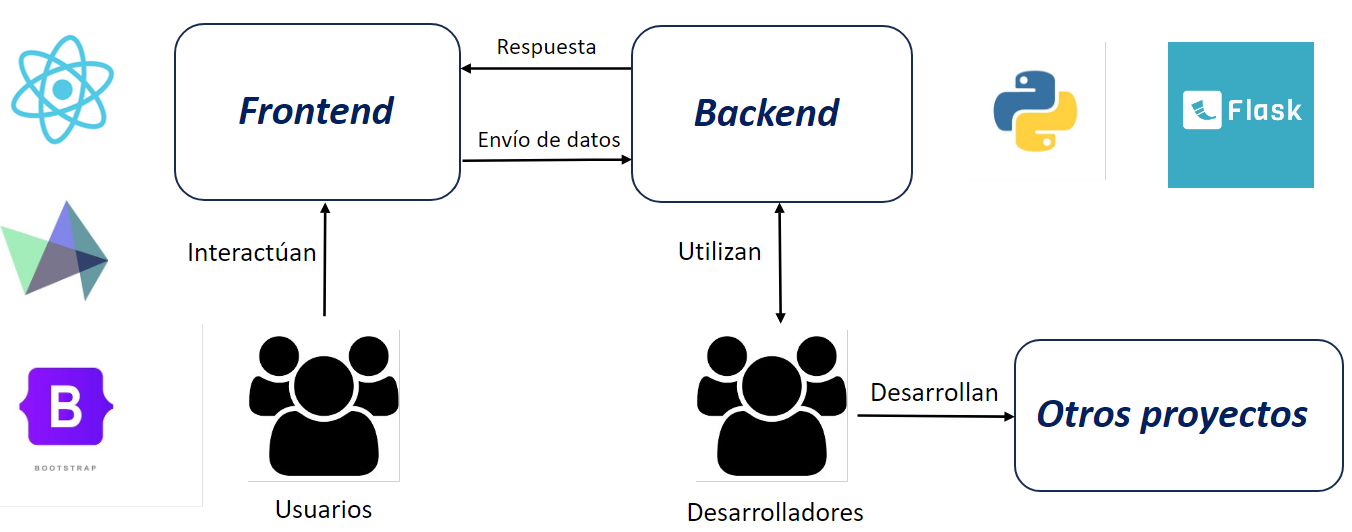
\includegraphics[width=\textwidth]{diagrama}
\end{figure}
\end{frame}
\section{Trabajo futuro}
\begin{frame}{Trabajo futuro}
\begin{itemize}
	\item Mejora de la interfaz de usuario.
	\item API tiempo meteorológico.
	\item Migrar el proyecto a microservicios.
	\item Diseñar algoritmos numéricos para resolver los sistemas tanto lineales como no lineales.
\end{itemize}
\end{frame}
\end{document}
